
%%%%%%%%%%%%%%%%%%%%%%%%%%%%%%%%%%%%%%%%%%%%%%%%%%%%%%%%%%%%%%%%%%%%%%%%%%%%%%%%%%
\chapter{Technical Designs}
\label{v1ch:tech-designs}
 
 
 
\section{LBNF Project}
 
LBNF will provide facilities at Fermilab and at SURF to enable the scientific program of DUNE. These facilities are geographically separated into the Near Site Facilities, those to be constructed at Fermilab, and the Far Site Facilities, those to be constructed at SURF. %They are summarized in sections below.
 
\subsection{Near Site Facilities}
 
The scope of LBNF at Fermilab is provision of the beamline plus the conventional facilities (CF) for this beamline as well as for the DUNE near detector. The layout of these facilities is shown in Figure~\ref{fig:nearsite-topo}. The science requirements as determined by the DUNE
Collaboration drive the performance of the beamline and near detector, which then provide requirements for the components, space, and functions necessary to construct, install, and operate the beamline and near detector. ES\&H and facility operations requirements (i.e., \textit{programmatic} requirements) also provide input to the design.
 
\begin{cdrfigure}[Layout of LBNF Near Site]{nearsite-topo}{Layout of LBNF Near Site}
  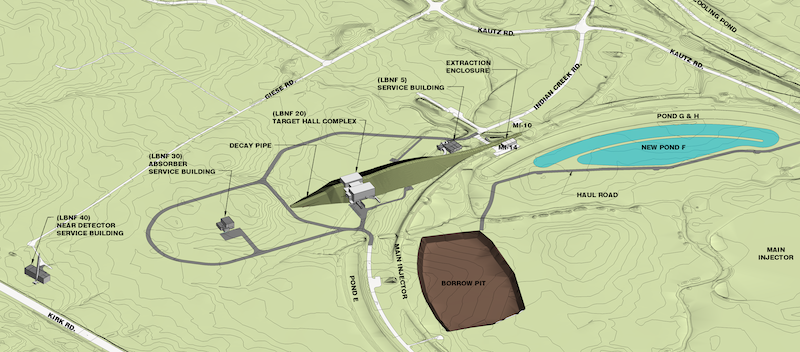
\includegraphics[width=\textwidth]{nearsite-topo}
\end{cdrfigure}
 
 
The beamline is designed to provide a neutrino beam of sufficient intensity and appropriate energy range to meet the goals of DUNE for long-baseline neutrino oscillation physics. The design is a conventional, horn-focused neutrino beamline. The components of the beamline will be designed to extract a proton beam from the Fermilab Main Injector (MI) and transport it to a target area where the collisions generate a beam of charged particles which decay into neutrinos to create the neutrino beam aimed at the near and far detectors.
 
The facility is designed for initial operation at proton-beam power of \SI{1.2}{\MW}, with the capability to support an upgrade to \SI{2.4}{\MW}. The plan is for twenty years of operation, while the lifetime of the Beamline Facility, including the shielding, is for thirty years. It is conservatively assumed that operations during the first five years will be at \MWadj{1.2} and the remaining fifteen years at \SI{2.4}{\MW}.  
The experience gained from the various neutrino projects has contributed extensively to the reference design. In particular, the NuMI beamline serves as the prototype design. Most of the subsystem designs and the integration between them follow, to a large degree, from previous projects. 
 
The proton beam will be extracted at a new point at MI-10. After extraction, this primary beam will establish a horizontally straight compass heading west-northwest toward the far detector, but will be bent upward to an apex before being bent downward at the appropriate angle. The primary beam is designed to be above grade to minimize expensive, underground construction; this also significantly enhances ground-water radiological protection. The design requires construction of an earthen embankment, or hill, whose dimensions are commensurate with the bending strength of the dipole magnets required for the beamline. 
 
The target marks the transition from the intense, narrowly directed proton beam to the more diffuse, secondary beam of particles that in turn decay to produce the neutrino beam. After collection and focusing, the pions and kaons that did not initially decay need a long, unobstructed volume in which to decay. This decay volume in the reference design is a pipe of circular cross section with its diameter and length optimized such that decays of the pions and kaons result in neutrinos in the energy range useful for the experiment. The decay volume is followed immediately by the absorber, which removes the remaining beam hadrons. 
 
Radiological protection is integrated into the LBNF beamline reference design in two important ways. First, shielding is optimized to reduce exposure of personnel to radiation dose and to minimize radioisotope production in ground water within the surrounding rock. Secondly, the handling and control of tritiated ground water produced in or near the beamline drives many aspects of the design. 
 
Beamline CF includes an enclosure connecting to the existing Main Injector at MI-10, concrete underground enclosures for the primary beam, targetry, horns, absorber, and related technical support systems. Service buildings will be constructed to provide support utilities the primary proton beam at LBNF~5 and to support the absorber at LBNF~30 (shown in Figure~\ref{fig:nearsite-topo}).  The Target Hall Complex at LBNF~20 houses the targetry system.  Utilities will be extended from nearby existing services, including power, domestic and industrial water, sewer, and communications. 
 
Near Detector CF includes a small muon alcove area in the Beamline Absorber Hall and a separate underground Near Detector Hall that houses the near detector. A service building called LBNF~40 with two shafts to the underground supports the near detector. The underground hall is sized for the reference near detector.
 
\subsection{Far Site Facilities}
 
The scope of LBNF at SURF includes both conventional facilities and cryogenic infrastructure to support the DUNE far detector. Figure~\ref{fig:lbnf-cavern-layout} shows the layout of the underground caverns that will house the detector modules with a separate cavern to house utilities and cryogenic systems. The requirements derive from DUNE Collaboration science requirements, which drive the space and functions necessary to construct and operate the far detector.  ES\&H and facility operations (programmatic) requirements also provide input to the design. The far detector is modularized into four \ktadj{10} fiducial mass detectors \fixme{determine if reference should be for total mass instead of fiducial}. The designs of the four detector pits in two caverns and the services to the caverns will be as similar to one another as possible for efficiency in design and construction as well as operation. 
 
\begin{cdrfigure}[LBNF Far Site cavern configuration]{lbnf-cavern-layout}{LBNF Far Site cavern configuration}  
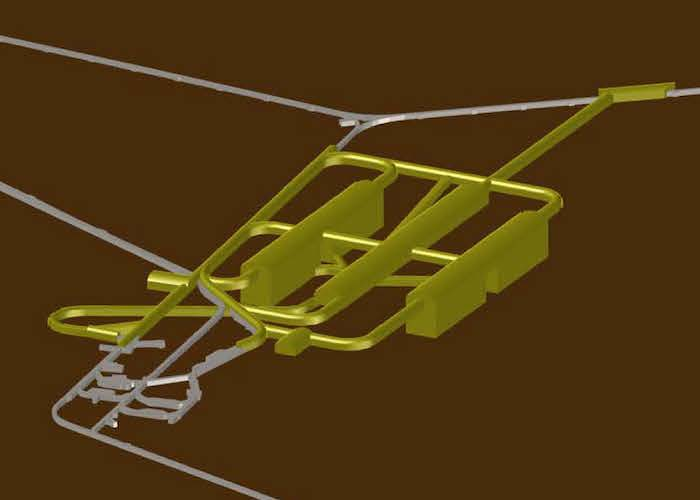
\includegraphics[width=.7\textwidth]{lbnf-cavern-layout}
\end{cdrfigure}
 
 
The scope of the Far Site CF includes design and construction for facilities both on the surface and underground. The underground conventional facilities includes new excavated spaces at the 4850L for the detector, utility spaces for experimental equipment, utility spaces for facility equipment, drifts for access, as well as construction-required spaces. Underground infrastructure provided by CF for the experiment includes power to experimental equipment, cooling systems and cyberinfrastructure. Underground infrastructure necessary for the facility includes domestic (potable) water, industrial water for process and fire suppression, fire detection and alarm, normal and standby power systems, a sump pump drainage system for native and leak water around the detector, water drainage to the facility-wide pump discharge system, and cyberinfrastructure for communications and security.
In addition to providing new spaces and infrastructure underground, CF will enlarge and provide infrastructure in some existing spaces for LBNF and DUNE use, such as the access drifts from the Ross Shaft to the new caverns. New piping will be provided in the shaft for cryogens (gas argon transfer line and the compressor suction and discharge lines) and domestic water as well as power conduits for normal and standby power and cyberinfrastructure. 
 
SURF currently has many surface buildings and utilities, some of which will be utilized for LBNF. The scope of the above-ground CF includes only that work necessary for LBNF, and not for the general rehabilitation of buildings on the site, which remains the responsibility of SURF. 
Electrical substations and distribution will be upgraded to increase power and provide standby capability for life safety. Additional surface scope includes a small control room in an existing building and a new building to support cryogen transfer from the surface to the underground near the existing Ross Shaft.
 
To reduce risk of essential but aging support equipment failure during the construction and installation period, several SURF infrastructure operations/maintenance activities are included as early activities in  the LBNF Project. These include completion of the Ross Shaft rehabilitation, rebuilding of hoist motors, and replacement of the Oro Hondo fan; if not addressed, this aging infrastructure could limit or remove access to the underground if equipment failed. 
 
The scope of the LBNF cryogenics infrastructure includes the design, fabrication, and installation of four cryostats to contain the liquid argon (LAr) and the detector components. It also includes a comprehensive cryogenic system that meets the performance requirements for purging, cooling and filling the cryostats, for achieving and maintaining the LAr temperature, and for purifying the LAr outside the cryostats. 
 
Each cryostat is composed of a free-standing steel-framed structure with a membrane cryostat vessel installed inside, to be constructed in one of the four excavated detector pits. The cryostat is designed to hold a total LAr mass capacity of 
17.1~kt. Each membrane tank cryostat has a stainless-steel liner as part of a full membrane system to provide full containment of the liquid cryogen. The hydrostatic pressure loading of the liquid cryogen is transmitted through rigid foam insulation to the surrounding structural steel frame which provides external support for the membrane. All penetrations into the interior of the cryostat will be made through the top plate to minimize the potential for leaks with the exception of the sidewall penetration for connection to the LAr recirculation system.
 
Cryogenic system components are located both on the surface and within the cavern. The cryogen receiving station is located on the surface near the Ross Shaft to allow for receipt of LAr deliveries for the initial filling period, as well as a buffer volume to accept liquid argon during the extended fill period. A large vaporizer for the nitrogen circuit feeds gas to one of four compressors located in the Cryogenic Compressor Building; the compressor discharges high pressure nitrogen gas to pipes in the Ross shaft. The compressors are located on the surface because the electrical power requirement and cooling requirement is much less than for similar equipment at the 4850L.  
 
Equipment at the 4850L includes the nitrogen refrigerator, liquid nitrogen vessels, argon condensers, external liquid argon recirculation pumps, and filtration equipment. Filling each cryostat with LAr in a reasonable period of time is a driving factor for the refrigerator and condenser sizing.  Each cryostat will have its own argon recondensers, argon-purifying equipment and overpressure protection system located in the Central Utility Cavern. Recirculation pumps will be placed outside and adjacent to each cryostat to circulate liquid from the bottom of the tank through the purifier.
 
 
\section{Strategy for Developing the LBNF Beamline}
 
The neutrino beamline described in this CDR is a direct outgrowth of the design~\cite{lbnecdr} developed for the 
CD 1 in 2012.  That design was driven by the need to minimize cost, while delivering the performance required to meet the scientific objectives of the long-baseline neutrino program.  It includes many features that followed directly from the 
successful NuMI beamline design as updated for the NOvA experiment.  It utilizes a target and horn system based on NuMI designs, with the spacing of the target and two horns set to maximize flux at the first, and to the extent possible, second 
oscillation maxima, subject to the limitations of  the NuMI designs for these systems.  The target chase volume --- length and width --- are set to the minimum necessary to accommodate this focusing system, and the temporary morgue space to store 
used targets and horns is sized based on the size of the NuMI components.  Following the NuMI design, the decay pipe is helium-filled, while the target chase is air-filled.  
 
The LBNF beamline is designed to utilize the Main Injector proton beam with energy between 60 and 120~GeV and beam power from 1.0 to 1.2~MW respectively, as will be delivered after the PIP-II upgrades~\cite{pip2-2013}.  The ability to vary the 
proton beam energy is important for optimizing the flux spectrum and to understand systematic effects in the beam production, and to provide flexibility to allow the facility to address future questions in neutrino physics which may require a 
different flux spectrum.  To allow for higher beam power that may be enabled by future upgrades to the Fermilab accelerator complex beyond PIP-II, those elements of the beamline and supporting conventional facilities that cannot be changed once 
the facility is built and has been irradiated are designed to accommodate beam power in the range of 2.0 to 2.4~MW for proton beam energy of 60 to 120~GeV.  These elements include the primary beam, target hall, decay pipe and absorber, as 
well as the shielding for them.  Components that can be replaced, such as targets and horns, are designed for the \MWadj{1.2} initial operation.  In general, additional R\&D, which is not part of the LBNF Project, is required to develop those components to be able to operate at the higher beam power.
 
Since the 2012 CD-1 review, the beamline design has evolved in a number of areas, as better understanding of the design requirements and constraints has been developed.  Some of these design changes have come to full maturity and are 
described in this CDR.  Others require further development and evaluation to determine if and how they might be incorporated into the LBNF neutrino beamline design.  They offer the possibility of higher performance, flexibility in 
implementation of future ideas, or greater reliability. The beamline facility is designed to have an operational lifetime of 20 years, and it is important that it be designed to allow future upgrades and modifications that will allow it to 
exploit new 
technologies and/or adapt the neutrino spectrum to address new questions in neutrino physics over this long period. The key alternatives and options under consideration and the strategy for evaluating and potentially implementing them are summarized here.  They are described in more detail elsewhere in this CDR or its Annexes.  
               
 
Further optimization of the target-horn system has the potential to substantially increase the neutrino flux at the first and especially second oscillation maxima and to reduce wrong-sign neutrino background, thereby increasing the sensitivity to CP 
violation and mass hierarchy determination, as discussed in \volphys.  The optimization work there is ongoing and may yield further improvements beyond those currently achieved. Engineering studies of the proposed horn designs and methods 
of integrating the target into the first horn must be performed to turn these concepts into real buildable structures that satisfy other requirements such as reliability and longevity.  These studies will be carried out between CD-1 and CD-2 to 
determine the baseline design for the LBNF target-horn system.  Since targets and horns must be replaceable, it is also possible to continue development of the target-horn system in the future and replace the initial system with a more advanced 
one or one optimized for different physics.  Such future development, beyond that necessary to establish the baseline design at CD-2, would be done outside of the LBNF Project.
 
The more advanced focusing system, called the ``optimized beam configuration'' in \volphys, utilizes horns that are longer and larger in diameter and that are spaced farther apart than the reference design, which would require a target chase approximately 9~m longer and 0.6~m wider 
than the reference design.  It cannot be ruled out that further optimization, or or future designs to explore new questions may require additional space beyond this.  Also, the larger horns will require larger 
space for temporary storage of used, irradiated components, requiring, in turn, an increase in the size of the morgue or a revision of the remote handling approach.  Between CD-1 and CD-2, studies will be done to determine not only the geometric 
requirements from the final baseline target-horn system, but also to estimate the dimensions needed to accommodate potential future designs.
 
The material, geometry and the structure of the target assembly itself can have significant impact both on the effective pion production and the energy spectrum of pions, which in turn affect the neutrino spectrum, and on the reliability and longevity of 
the target, which affects the integrated beam exposure.  Potential design developments range from incremental (e.g., changing from the reference design rectangular cross section, water-cooled graphite target to a cylindrical 
helium-cooled target), to more substantial (e.g., changing target material from graphite to beryllium), to radical (e.g., implementing a hybrid target with lighter material upstream and heavier material downstream and perhaps constructed of a set of spheres captured in a 
cylindrical skin).  New designs beyond the current reference design are also needed in order to accommodate the higher beam power (up to 2.4~MW) that will be provided by the PIP-II upgrade.  Target development will largely be carried out in the 
context of worldwide collaborations on high-power targetry such as the Radiation Damage In Accelerator Target 
Environments (RaDIATE) collaboration, and not within the LBNF Project. The LBNF design must be such that it can fully exploit future developments in target design.
 
The length and diameter of the decay pipe also affect the neutrino flux spectrum.  A longer decay pipe increases the total neutrino flux with a larger increase at higher energies; a larger diameter allows the capture and decay of lower-energy pions, 
increasing the neutrino flux at lower energy as described in \volphys. The dimensions also affect the electron-neutrino and wrong-sign backgrounds.  Unlike targets and horns, the decay pipe cannot be modified after the facility is built, making the 
choice of geometry particularly important.  The reference design values of \SI{204}{\meter} length and \SI{4}{\meter} diameter appear well matched to the physics of DUNE but studies to determine the optimal dimensions continue.  The cost of increasing the decay 
pipe length or diameter  is relatively large, including 
the impact on the absorber.
Therefore, studies of the decay pipe must include 
evaluation of the relative advantages of
investment in the decay pipe versus investment in 
other systems, e.g., a larger target hall complex, more advance target-horn systems, or more far detector mass.  Ongoing studies will continue to be carried out jointly by LBNF and DUNE between CD-1 and CD-2 to determine the baseline decay pipe geometry.


\section{The DUNE Detectors}

The DUNE detectors to be installed at SURF (the far location) and FNAL (the near location) will enable the scientific program of DUNE.  The detector 
requirements derive from these DUNE science goals.

\subsection{The Far Detector}
The  Far Detector (FD) will be located deep underground at the 4850L and have
a  fiducial mass of \ktadj{40} to perform sensitive studies of long-baseline oscillations with a \kmadj{1300} baseline as well as a rich astroparticle physics programme and nucleon decay searches. The FD  will be composed of four %identical 
similar modules, each instrumented as a Liquid Argon Time Projection Chamber (LArTPC).
The concept of the LArTPC provides
excellent tracking and calorimetry performance, hence it is ideal for massive neutrino detectors such as DUNE's, which require a high signal efficiency and effective background discrimination,  an excellent capability to identify and  precisely measure neutrino events over a wide range of energies, and an excellent reconstruction of the kinematical properties
with a high resolution. The full imaging of events will allow study of neutrino interactions and
other rare events in an unprecedented way. \fixme{to an unprecedented level of precision?}
 The huge mass will allow collectiopn of sufficient statistics for precision
studies, as discussed in Chapter~\ref{v1ch:science}.

The LArTPC, pioneered in the context of the ICARUS project, is a mature technology. It is the outcome
of several decades of R\&D executed worldwide.  Nonetheless, the size of a single \ktadj{10} DUNE module represents an extrapolation by approximately one order of magnitude compared to the largest operated detector, the ICARUS~T600. To address this challenge, DUNE is developing two far detector options, the reference design and the alternative design, and is engaged in a 
comprehensive prototyping effort. At this stage, the development of two FD options is a strength and an added-value \fixme{asset or advantage?}
made possible by the merging of the worldwide neutrino community into DUNE.  The two detector
concepts are illustrated in Figure~\ref{fig:FarDet-overview-SPDP}.

\begin{cdrfigure}[3D models of the DUNE far detector designs]{FarDet-overview-SPDP}
{3D models of two 10-kt detectors using the single-phase reference design (left) 
and the dual-phase alternative design (right) for the DUNE far detector to be 
located at 4850L.}
\centering
\begin{minipage}[b]{1.0\textwidth}
\begin{center}
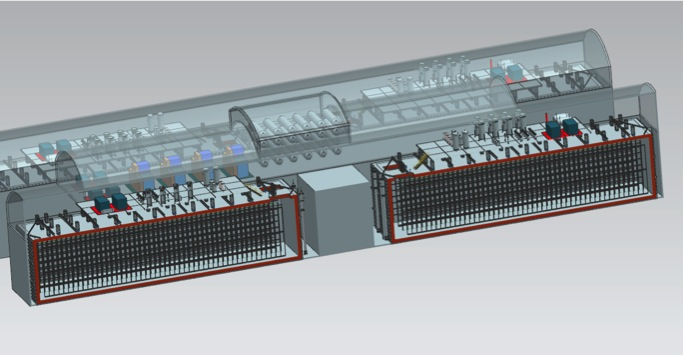
\includegraphics[width=.5\textwidth]{FarDet-3D-SP.jpg}
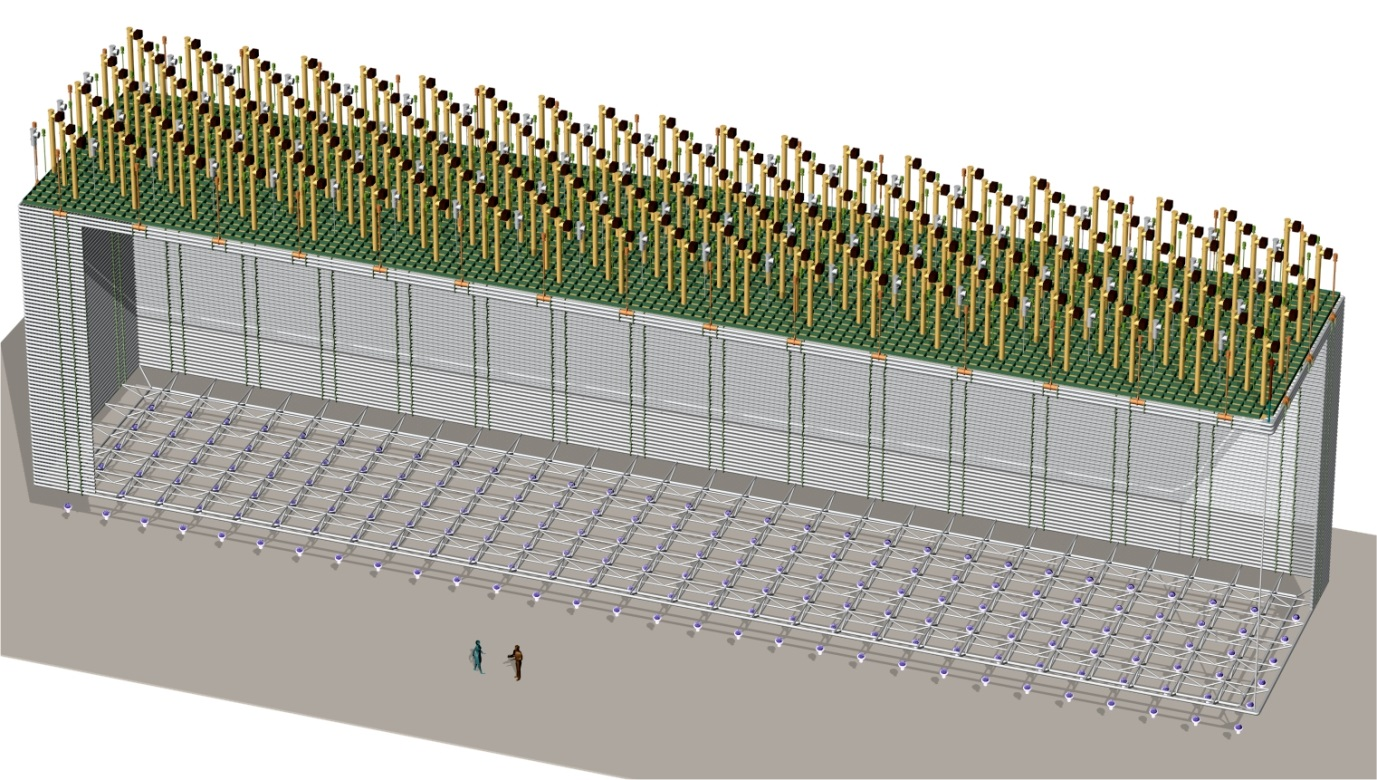
\includegraphics[width=0.46\textwidth]{DP_det2.jpg}
\end{center}
\end{minipage}
\end{cdrfigure}


Interactions in LAr produce ionization charge and scintillation light.
The charge is drifted with a constant electric field away from the cathode
plane and towards the segmented anode plane. \fixme{Maury had comments on this; I think it's that the negative charge, i.e., ionization electrons that are drifted away from cathode, not charge in general}
The prompt scintillation light,
detected by photo-detectors, provides the absolute time of the event.
The reference design adopts a single-phase readout, where the readout anode is composed wire planes in the LAr volume. 
In the alternative design, the  dual-phase approach is considered, in which the 
ionization charges are extracted, amplified and detected in gaseous argon (GAr) above the liquid surface. 
The dual-phase design would allow for a finer readout pitch (3~mm), 
a lower detection-energy threshold, and better pattern reconstruction of the events.
%The reference and alternative designs adopt complementary design to collect the scintillation light.
The photon-detection scheme used in both designs is similar. \fixme{Anne changed sentence}

The \ktadj{10} reference design TPC is described in Chapter 4 of \voldune. 
Its active volume is 12\,m high, 14.5\,m wide and 
58\,m long, instrumented with APAs, 
which are 6\,m high and 2.3\,m in width, and CPAs, 3\,m high by 2.5\,wide. Vertical stacks of
two APAs and four CPAs %are stacked vertically to 
instrument 
the 12\,m height of the active volume. The 12.5-m width of the detector is 
spanned by three stacks of APAs and two stacks of CPAs in an APA:CPA:APA:CPA:APA
arrangement, resulting in four 3.6\,m drift volumes, while the 58-m length of the active volume
is spanned by 25 such stack arrangements placed edge to edge. Hence a \ktadj{10} 
far detector module consists of 150 APAs and 200 CPAs. The CPAs are held a -180\,kV, such that 
ionization electrons drift a maximum distance of 3.6\,m in the electric field of 500\,V\,cm$^{-1}$.
The highly modular nature of the detector design allows for manufacturing to be distributed across a number of sites.

A  comprehensive prototyping strategy for both designs is actively pursued.
The reference design, closer to the original ICARUS design, is currently being validated in the 35-t prototype 
LAr detector at Fermilab.  The alternative design, representing a novel approach, has been proven on several
small-scale prototypes. Presently
a 20-t dual-phase prototype with dimensions 3$\times$1$\times$1~m$^3$ is being constructed at CERN (WA105),  
and should be operational in 2016. 
The ultimate validation of the engineered solutions for both designs of the FD is foreseen at 
the CERN Neutrino Platform around 2018, \fixme{is it a place or a program?} where full-scale engineering prototypes will be 
assembled and commissioned. Following this milestone, a test-beam data 
campaign will be executed %in the following years 
to collect a large sample of charged-particle interactions
in order to study the response of the detector with high precision.
A comprehensive list of synergies between the reference and alternative designs has been identified (Chapter 6 of \voldune). Common solutions for DAQ, electronics, HV feed-throughs, and so on, will pursued and implemented, independent of the details of the TPC design. The ongoing and planned efforts %and those at the CERN Neutrino Platform 
will
provide the ideal environment to exploit such synergies and implement common solutions.
There is recognition that the LArTPC technology will continue to evolve with (1) the large-scale prototypes at the CERN Neutrino Platform and the experience from the Fermilab SBN program, and (2) the experience gained during the construction and commissioning of the first \ktadj{10} module. 
The staged approach with the deployment of consecutive modules will
%give access to 
enable an early science program while allowing implementation of improvements and developments  during the experiment's lifetime.
The strategy for implementing
the far detector is presented in Chapter~\ref{v1ch:strategy}.

%%%%%%%%%%%%%%%%%%%%%%%%%%%%%%%%%%%%%%%%%%
\subsection{The Near Detector} %s} <--- I think there's only one overall near detector, right?

\fixme{We need to distinguish between near detector and near neutrino detector. I think the ND is NND+BLM+DAQ. Is this right?}

To meet the systematic precision needed to fulfill the DUNE science objectives, the near detector must thoroughly 
characterize the neutrino beam at the source, where it is composed of both muon- and electron-flavored neutrinos and antineutrinos. \fixme{Did I get this right?}  Additionally, it must precisely measure the cross sections and the particle yields of various processes that compose neutrino events.
 %
Its primary role is therefore collection of neutrino-interaction statistics to an uprecedented level. This wealth of fundamental neutrino-interaction 
measurements will satisfy important secondary scientific goals of the DUNE Collaboration. 
%
The reference design for the neutrino near detector (NND) design is the NOMAD-inspired fine-grained tracker (FGT), illustrated in Figure~\ref{fig:FGT_schematic}. The subsystems of the NND include a central 
straw-tube tracker and an electromagnetic calorimeter embedded in a 0.4-T dipole field. The steel of the
magnet yoke will be instrumented with muon identifiers. The strategy for implementation of
the Near Detector \fixme{ND or NND?} is presented in Chapter~\ref{v1ch:strategy}.

\fixme{The above is a rewrite of the following pgraph (so of course I propose dropping the following). Anne}
The spectrum and flavor composition of the neutrino beam will be measured with high precision 
in order to reach the ultimate sensitivity for the long-baseline neutrino oscillation studies.
The separation between fluxes of neutrinos and antineutrinos requires a magnetized neutrino detector to 
charge-discriminate electrons and muons produced in the neutrino charged-current interactions.
This is the primary role of the DUNE near detector system, however, being exposed to an intense flux of neutrinos
will also provides the opportunity to collect an unprecedentedly high statistics of neutrino 
interactions  for an extended science program. 
The near detector will therefore provide an opportunity for a wealth of fundamental neutrino interaction 
measurements, which are an important part of the secondary scientific goals of the DUNE collaboration. 
The reference design for the neutrino near detector (NND) design is the NOMAD-inspired fine-grained tracker (FGT), illustrated in Figure~\ref{fig:FGT_schematic}. The subsystems of NND comprise a central 
straw-tube tracker and an electromagnetic calorimeter embedded in a 0.4-T dipole field. The steel of the
magnet yoke will be instrumented with muon identifiers. The strategy to implement
the Near Detector is presented in Chapter~\ref{v1ch:strategy}.


\begin{cdrfigure}[A schematic drawing of the fine-grained
tracker design]{FGT_schematic}{A schematic drawing of the fine-grained tracker design}
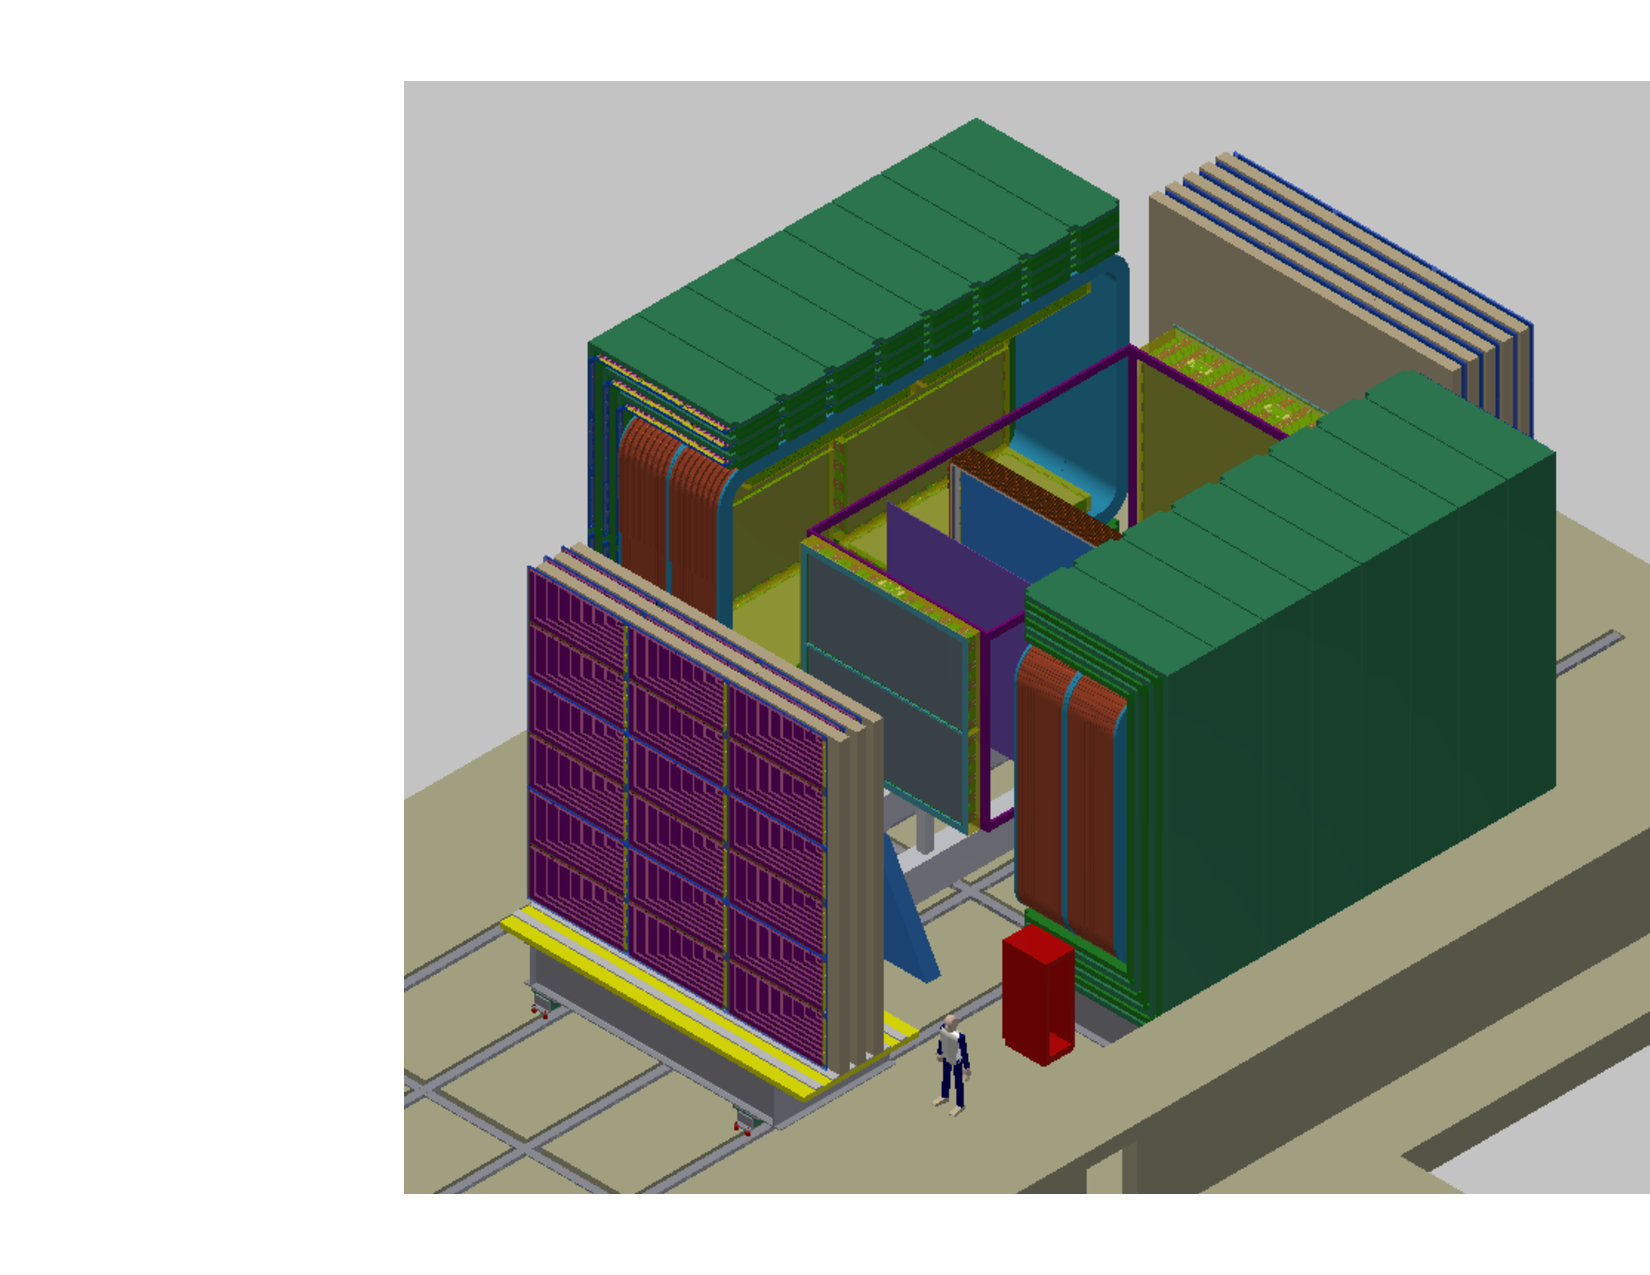
\includegraphics[width=.8\textwidth]{FGT_Overview}
\end{cdrfigure}


The NND will be complemented by a Beamline Measurement System (BLM) located in the region of the beam absorber at the downstream end of the decay region. The BLM aims to measure the muon fluxes from hadron decay and
 is intended to monitor the beam profile on a spill-by-spill basis. It will operate for the life of the experiment.


\section{Strategy for Implementing the DUNE Far Detector}

\fixme{Some dates in this section are being revised as the resource-loaded schedule is matched to DOE funding guidance. Revised dates are expected soon.}


The LBNF project will provide four separate cryostats to be located on the 4850L at the 
Sanford Underground Research Facility (SURF).  Instrumentation of the first cryostat 
will commence in 20yy. %2021/2022 
As part of the deployment and risk mitigation strategy, 
the cryostat for the second detector must be available when the first cryostat 
is filled. The aim is to install third and fourth cryostats as rapidly thereafter as funding 
allows.

The DUNE collaboration aims to deploy four 10-kt (fiducial) mass FD modules based 
on the Liquid Argon Time Projection Chamber (LArTPC) technology. The viability 
of the basic LArTPC technology has been proven by the ICARUS experiment. Neutrino 
interactions in liquid argon produce ionization and scintillation signals. While 
the basic detection method is the same, DUNE contemplates two options for the readout 
of the ionization signals: single-phase readout, where the ionization is detected 
using readout (wire) planes in the liquid argon volume; and the dual-phase approach, where 
the ionization signals are amplified and detected in gaseous argon above the liquid 
surface. The dual-phase approach, if demonstrated, would allow for a 3-mm readout 
pitch, a lower detection energy threshold, and potentially better reconstruction of 
the events. The DUNE single-phase readout design is being validated 
in the 35-t prototype detector at Fermilab. A 20-t dual-phase readout prototype is being 
constructed at CERN and will operate in 2016. An active development program for 
both technologies is being pursued in the context of the Fermilab Short-Baseline Neutrino (SBN)
program and 
the CERN Neutrino Platform. 
%Currently, the development of the dual-phase technology 
%is being funded from outside the DOE project. 
A flexible 
approach to the DUNE far detector designs offers the potential to bring additional 
interest and resources into the experimental collaboration. 

\subsection{Guiding Principles for the DUNE Far Detector}

\begin{itemize}
\item The lowest-risk design for the first 10-kt module satisfying the requirements 
will be adopted, allowing for its installation at SURF to commence in 20yy. %2021/2022. 
Installation  of the second 10-kt module should commence before 20yy. % 2023.

\item  Recognition that the LArTPC technology will continue to evolve with: (1) the 
large-scale prototypes at the CERN Neutrino Platform and the experience from the 
Fermilab SBN program, and (2) the experience gained during the construction and 
commissioning of the first 10-kt module. It is assumed that all four modules 
will be similar but not necessarily identical.

\item  In order to start installation on the timescale of 20yy, % 2021/2022,
the first  10-kt module will be based on the APA/CPA design, which is currently the lowest
risk option. There will be a clear and transparent decision process (organized by the DUNE 
technical board) for the design 
of the second and subsequent far detector modules, allowing for evolution of the 
LArTPC technology to be implemented. The decision will be 
based on physics performance, technical and schedule risks, costs and funding 
opportunities.

\item The DUNE Collaboration will instrument the second cryostat as soon as possible.

\item A comprehensive list of synergies between the reference and alternative designs 
has been identified and summarized in \voldune. Common solutions for DAQ, 
electronics, HV feed-throughs, etc., will be pursued and implemented, independent 
of the details of the TPC design.

\end{itemize}

\subsection{Strategy for the First 10-kt Far Detector TPC}



The viability of wire-plane LArTPC readout has already been demonstrated by the ICARUS T600 
experiment, where data were successfully accumulated over a period of three years. 
An extrapolation of the observed performance and the implementation of improvements 
in the design (such as immersed cold electronics) will allow the single-phase 
approach to meet the LBNF/DUNE far detector requirements. In order to start the FD installation
by 20yy, % 2022, 
the first 10-kt module will be based on the single-phase design using anode and cathode
plane assemblies (APAs and CPAs), described in Chapter 4 of \voldune. 
Based on previous experience and the 
future development path in the Fermilab SBN program and at the CERN Neutrino Platform, 
this choice represents the lowest-risk option for installation of the first 10-kt FD module by 
20yy. % 2021/2022. 
For these reasons, the APA/CPA single-phase wire plane LArTPC readout 
concept %, described in Volume 4 of the DUNE CDR, 
is the \textit{reference design} 
for the far detector. 
The design is already relatively advanced for the conceptual  
stage. From this point on, modifications to the reference design will require approval
by the DUNE Technical Board. A preliminary design review will take place as early 
as possible, utilizing the experience from the DUNE 35-t prototype; the design 
review will define the baseline design that will form the basis of the TDR (CD-2). 
At that point, the design will be put under a formal change-control 
process. 

A single-phase engineering prototype,
comprising six full-sized drift cells of the TDR engineering baseline,
will be validated at the CERN neutrino platform in 2018 (pending approval by CERN). 
This %single-phase engineering prototype at CERN 
prototype is a central part of the risk-mitigation 
strategy for the first 10-kt module and is part of the DOE-funded portion of the DUNE project. 
Based on the  performance of this prototype at the CERN Neutrino Platform, a final design review will 
take place towards the end of 2018 and construction of the readout planes will 
commence in 2019, to be ready for first installation in 20yy. % 2021/2022. 
The design reviews 
will be organized by the DUNE Technical Coordinator. 

In parallel with preparation for construction of the first 10-kt far detector module, 
\fixme{Do we want to use FD and ND or spell them out each time?}
the DUNE collaboration recognizes the potential of the dual-phase technology and 
strongly endorses the already approved development program at the CERN Neutrino 
Platform (the WA105 experiment), which includes the operation of the 20-t prototype 
in 2016 and the 6$\times$6$\times$6\,m\textsuperscript{3} demonstrator in 2018. Participation 
in the WA105 experiment is open to all DUNE collaborators. A concept for the dual-phase 
implementation of a far detector module is presented as an \textit{alternative 
design} in \voldune. This alternative design, if demonstrated, 
could form the basis of the second or subsequent 10-kt modules, in 
particular to achieve improved detector performances in a cost-effective way. 

\subsection{DUNE at the CERN Neutrino Platform}

WA105 has signed an MoU with the CERN Neutrino Platform to provide a large \textasciitilde{} 
8$\times$8$\times$8\,m\textsuperscript{3} cryostat by October 2016 in the new EHN1 extension, 
and it is foreseen that a second large cryostat to house the single-phase LArTPC will 
be provided on a similar timescale. Both will be exposed to charged-particle test 
beam spanning a range of particle types and energies.   

The DUNE collaboration will instrument one of these cryostats with an arrangement 
of six APAs and six CPAs, in a APA:CPA:APA configuration providing an engineering 
test of the full-size drift volume. These will be produced at two or more sites with the cost 
shared between the DOE project and international partners. The CERN prototype thus 
provides the opportunity for the production sites to validate the manufacturing 
procedure ahead of large-scale production for the far detector. Three major operational 
milestones are defined for this single-phase prototype: (1) engineering validation 
--- successful cool-down;( 2) operational validation --- successful TPC readout with 
cosmic-ray muons; and (3) physics validation with test-beam data. Reaching milestone 
2, scheduled for early 2018, will allow the retirement of a number of technical 
risks for the construction of the first 10-kt module. The proposal for the DUNE 
single-phase prototype will be presented to the CERN SPSC in June 2015. 

In parallel, the WA105 experiment approved by the CERN Research Board in 2014 and supported 
by the CERN Neutrino Platform has a funded plan to construct and operate a large-scale 
demonstrator utilizing the dual-phase readout in the test beam by October 2017. 
Successful operation and demonstration of long-term stability of the WA105 demonstrator 
will establish this technological solution as an option for the second or subsequent 
far detector modules. The DUNE dual-phase design is based on independent 3$\times$3\,m$^2$
charge readout planes (CRP) placed at the gas-liquid interface. Each module provides 
two perpendicular ``collection'' views with 3-mm readout pitch. A 10-kt module 
would be composed of 80 CRPs hanging from the top of the cryostat, decoupled from 
the field cage and cathode. The WA105 demonstrator will contain four 3$\times$3m$^2$ 
CRPs of the DUNE type giving the opportunity to validate the manufacturing procedure 
ahead of large-scale production. WA105 is presently constructing a 3$\times$1\,m$^2$ 
CRP to be operated in 2016. The same operational milestones (engineering, operational, 
physics) are defined as for the single-phase prototype.

The DUNE program at the CERN Neutrino Platform will be coordinated by a single 
L2 manager. Common technical solutions will be adopted wherever possible for the 
DUNE single-phase engineering prototype and the dual-phase (WA105) demonstrator. 
The charged-particle test-beam data will provide essential calibration samples 
for both technologies and will enable a direct comparison of the relative physics 
capabilities of the single-phase and dual-phase TPC readout. 

\subsection{Strategy for the Second and Subsequent 10-kt Far Detector Modules}

For the purposes of cost and schedule, the reference design for the first module 
is taken as the reference design for the subsequent three modules. However, 
the experience with the first 10-kt module and the development activities at 
the CERN Neutrino Platform are likely to lead to the evolution of the TPC technology, both 
in terms of refinements to single-phase design and the validation of the operation 
of the dual-phase design. The DUNE technical board will instigate a formal review 
of the design for the second module in 20yy; %2020; 
the technology choice 
will be based on risk, cost (including the potential benefits of additional 
non-DOE funding) and physics performance (as established in the CERN charged-particle 
test beam). After the decision, the design of the second module will come under formal 
change control. This process will be repeated for the third and fourth modules 
in 20yy.%2022.

This strategy allows flexibility with respect to international contributions, 
enabling the DUNE collaboration to
adopt evolving approaches for subsequent modules. This approach provides the possibility of attracting interest 
and resources from a broader community, and space for flexibility to respond to 
the funding constraints from different sources. 

\section{Strategy for Implementing the DUNE Near Detector(s)}

The LBNF project will provide the facilities for the DUNE near detector systems 
(muon monitors and near neutrino detector). The primary scientific motivation for 
the DUNE near detector system is to determine the beam spectrum for the long-baseline 
neutrino oscillation studies. The near detector, which is exposed to an intense 
flux of neutrinos, also enables a wealth of fundamental neutrino 
interaction measurements, which are an important part of the  scientific 
goals of the DUNE collaboration. Within the former LBNE collaboration the neutrino 
near detector (NND) design was the NOMAD-inspired fine-grained tracker (FGT), which 
was established through a strong collaboration of U.S. and Indian institutes.

\subsection{Guiding Principles for the DUNE Near Detector}

\begin{itemize}
%%\item Recognition of the central importance of the reference design for NND;  
\item  The primary design consideration of the DUNE neutrino near detector is the 
ability to adequately constrain the systematic errors in the DUNE LBL oscillation 
analysis; this requires the capability to precisely measure exclusive neutrino
interactions.

\item An additional design consideration for the DUNE NND is the self-contained non-oscillation 
neutrino physics program.

\item It is recognized that a detailed cost-benefit study of potential near detector options 
has yet to take place and such a study is of high priority to the DUNE project. \fixme{DUNE Project or Collaboration?}
\end{itemize}

\subsection{The DUNE Near Detector Reference Design }

The NOMAD-inspired fine-grained tracker (FGT) concept is the \textit{reference 
design} for CD-1 review. The cost and resource-loaded schedule for CD-1 review 
will be based on this design, as will the near site conventional facilities. The 
Fine-Grained Tracker consists of:  central straw-tube tracker (STT) of volume 
3.5\,m$\times$3.5\,m$\times$6.4\,m; a lead-scintillator sandwich sampling electromagnetic calorimeter 
(ECAL); a large-bore warm dipole magnet, with inner dimensions of 
4.5\,m$\times$4.5\,m$\times$8.0\,m, surrounding the STT and ECAL and providing a magnetic field of 0.4\,T; 
and RPC-based muon detectors (MuIDs) located in the steel of the magnet, as well 
as upstream and downstream of the STT. The reference 
design is presented in Chapter 
7 of \voldune. 

For ten years of operation in the LBNF 1.2-MW beam (5 years neutrinos + 5 years 
antineutrinos), the near detector will record a sample of more than 100 million 
neutrino interactions and 50 million antineutrino interactions. These vast samples 
of neutrino interactions shall provide the necessary strong constraints on the 
systematic uncertainties for the LBL oscillation physics --- the justification is 
given in Section 6.1.1 of Volume \volphys. The large samples of neutrino 
interactions will also provide significant physics opportunities, including 
numerous topics for PhD theses.  

\subsection{DUNE Strategy for the Near Detector}

The contribution of Indian institutions to the design and construction of the DUNE 
FGT neutrino near detector is a vital part of the strategy for the construction 
of the experiment. The reference design will provide a rich self-contained physics 
program. From the perspective of an ultimate LBL oscillation program, there may 
be benefits of augmenting the FGT with, for example, a relatively small LArTPC 
in front of the FGT that would allow for a direct comparison with the far detector. 
A second line of study would be to augment the straw-tube tracker  with 
a High-Pressure Gaseous Argon TPC. At this stage, the benefits of such options 
have not been studied; alternative designs for the NND are not presented in 
the CDR and will be the subject of detailed studies in the coming months. 

\subsection{DUNE Near Detector Task Force}

A full end-to-end study of the impact of the FGT NND design on the LBL oscillation 
systematics has yet to be performed. Many of the elements of such a study are in 
development, for example the Monte Carlo simulation of the FGT and the adaptation 
of the T2K framework for implementing ND measurements as constraints in the propagation 
of systematic uncertainties to the far detector. 

After the CD-1-R review, the DUNE collaboration will initiate a detailed study 
of the optimization of the NND system. To this end a new task force will be set 
up with the charge of:

\begin{itemize}
\item delivering the simulation of the NND reference design and possible alternatives

\item undertaking an end-to-end study to provide a quantitative understanding of 
the power of the NND designs to constrain the systematic uncertainties on the LBL 
oscillation measurements

\item quantifying the benefits of augmenting the reference design with a LArTPC 
or a high-pressure gaseous argon TPC
\end{itemize}

High priority will be placed on this work and the intention is to engage a broad 
cross section of the collaboration in this process. The task force will be charged 
to deliver a report by July 2016. Based on the report of this task force and input 
from the DUNE Technical Board, the DUNE Executive Board will refine the DUNE strategy 
for the near detector.


